\begin{frame}\begin{center}
{\LARGE\textbf{Paper}}
\end{center}\end{frame}
%-------------------------------------------------------------------------------
%-------------------------------------------------------------------------------
\begin{frame}
\begin{quote}\small
This paper estimates the rate of return to the HighScope Perry Preschool Program, an early intervention
program targeted toward disadvantaged African-American youth. Estimates of the rate of return to the Perry
program are widely cited to support the claim of substantial economic benefits from preschool education
programs. Previous studies of the rate of return to this program ignore the compromises that occurred in the
randomization protocol. They do not report standard errors. The rates of return estimated in this paper
account for these factors. We conduct an extensive analysis of sensitivity to alternative plausible
assumptions. Estimated annual social rates of return generally fall between 7 and 10\%, with most estimates
substantially lower than those previously reported in the literature. However, returns are generally
statistically significantly different from zero for both males and females and are above the historical return
on equity. Estimated benefit-to-cost ratios support this conclusion.
\end{quote}
\end{frame}
%-------------------------------------------------------------------------------
%-------------------------------------------------------------------------------
\begin{frame}
\begin{itemize}
\item\bibentry{Heckman.2010j}
\end{itemize}
Part of a whole sequence ...

{\scriptsize\begin{itemize}
\item\bibentry{Heckman.2011b}
\item\bibentry{Heckman.2010k}
\item\bibentry{Heckman.2017}
\end{itemize}}
\end{frame}
%-------------------------------------------------------------------------------
%-------------------------------------------------------------------------------
\begin{frame}\textbf{HighScope Perry Preschool Program}

\begin{itemize}
\item Perry Elementary School in Yipsilanti, Michigan in early 1960s
\item beginning at age three and lasting two years
\item 2,5 hours preschool program on weekdays during the school year
\item weekly home visits by teachers
\item curriculum based on supporting children's cognitive and socio-emotional development
\item follow-up interviews at age 15, 19, 27, and 40
\end{itemize}
\end{frame}
%-------------------------------------------------------------------------------
%-------------------------------------------------------------------------------
\begin{frame}\textbf{Challenges}
\begin{itemize}
\item the randomization was compromised
\item there are not data on participants past age 40 and it is necessary to extrapolate out-of-sample to obtain earnings profiles pat that age to estimate the lifetime impacts
\item some data are missing for participants prior to age 40
\item there is difficulty in assigning reliable values to non-market outcomes such as crime
\end{itemize}
\end{frame}
%-------------------------------------------------------------------------------
%-------------------------------------------------------------------------------
\begin{frame}\textbf{Selected Contributions}
\begin{itemize}
\item We account for compromised randomization in evaluating this program.
\item We develop standard errors for all our estimates of the rate of return.
\item We use state-of-the-art methods to extrapolate missing future earnings.
\end{itemize}
\end{frame}
%-------------------------------------------------------------------------------
%-------------------------------------------------------------------------------
\begin{frame}\begin{figure}
\scalebox{0.75}{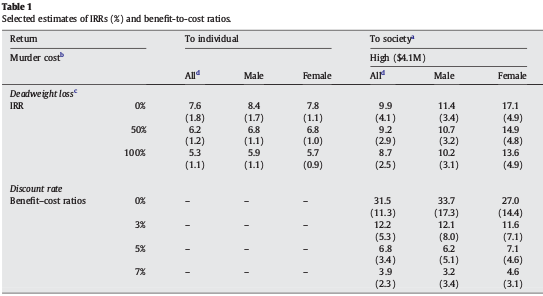
\includegraphics{fig-table-1}}
\end{figure}\end{frame}
%-------------------------------------------------------------------------------
%-------------------------------------------------------------------------------
\begin{frame}\begin{center}
\LARGE\textit{Public Impact}
\end{center}\end{frame}
%-------------------------------------------------------------------------------
%-------------------------------------------------------------------------------
\begin{frame}
\begin{quote}\Large
Every dollar we invest in high-quality early childhood education can save more than seven dollars later on -- by boosting graduation rates, reducing teen pregnancy, even reducing violent crime.
\end{quote}
\end{frame}
%-------------------------------------------------------------------------------
%-------------------------------------------------------------------------------
\begin{frame}\begin{figure}
\scalebox{0.30}{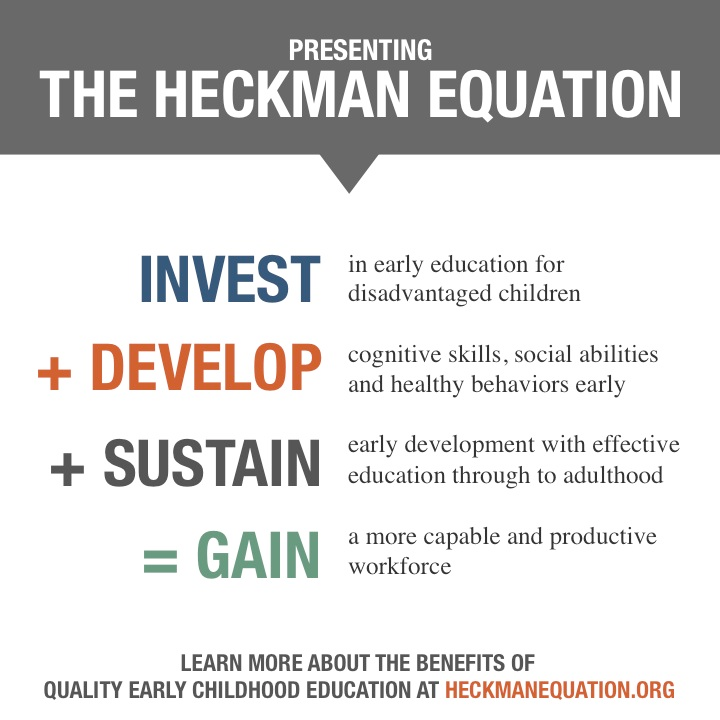
\includegraphics{fig-heckmanequation}}
\end{figure}\end{frame}
%-------------------------------------------------------------------------------
%-------------------------------------------------------------------------------
\begin{frame}
This handbook chapter provides the most recent overview on early childhood education.
\begin{itemize}
\item \bibentry{Elango.2016}
\end{itemize}
\end{frame}
%-------------------------------------------------------------------------------
%-------------------------------------------------------------------------------
